\documentclass{article}
\usepackage[utf8]{inputenc}
\usepackage[margin=1.0in]{geometry}
\usepackage{graphicx}
\usepackage{amsmath, amssymb}

\usepackage{hyperref}
%Import the natbib package and sets a bibliography style
\usepackage[square,numbers]{natbib}
\bibliographystyle{abbrvnat}

\title{Note of JC Lecture: Motor Parameter Identification}
\author{Lecture by Dr. Pilwon Hur}
\date{June 2015\footnote{Recorded by Kenneth Chao}}


\begin{document}

\maketitle

\section*{Nomenclature}
\begin{itemize}
\item[] $V$ (XXXvolt): voltage supplied on the motor
\item[] $V$ (XXXvolt): voltage supplied on the motor
\item[] $R$ (ohm): resistance of the motor
\item[] $L$ (henry): inductance of the motor
\item[] $i$ (amp): current going through the motor
\item[] $\theta$ (rad): rotation angle of motor rotor
\item[] $\dot\theta$ or$\omega$ (rad/$s$): angular velocity of motor rotor
\item[] $J$ ($kg\cdot m^2$): inertia of motor rotor
\item[] $B$ ($Nm\cdot s/m$): damping of motor
\item[] $K_b$: ($rad/s\cdot volt$): velocity constant of motor
\item[] $K_t$: ($Nm/amp$): torque constant of motor
\item[] $T$ ($Nm$): toque generated by motor
\item[] $\tau$ (sec): time constant of 1st order system
\item[] $V_s$ (volt): voltage across the small resistance for current measurement
\item[] $R_s$ (ohm): resistance of the small resistance for current measurement
\end{itemize}
\section{Brushed DC motor}
In general, brushed DC motor is easy to control in the sense of the related hardware implementation and its simple linear characteristics on both electrical and mechanical parts. But since the brushes wear down and require replacement, brushless DC motors using power electronic devices have displaced brushed motors from many applications \cite{WikiDCM}.
\subsection{Generic DC Motor Model}
\begin{figure}[h!]
\centering
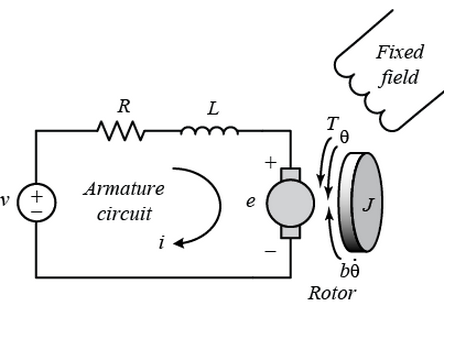
\includegraphics[scale=0.6]{Motor.png}
\caption{The Motor model \cite{MotorFig} }
\label{fig:Motor_Model}
\end{figure}
A generic brushed DC motor system (as shown in Figure \ref{fig:Motor_Model}) can be expressed as follows:
\begin{align}
\label{eqn:Electro}
V=Ri_+L\frac{di}{dt}+K_b\cdot \dot{\theta}\\
\label{eqn:Mechanics}
J\ddot{\theta}+B\dot{\theta}=T=K_t\cdot i,
\end{align}
where $R$ and $L$ are the resistance and inductance of motor, $J$ is the inertia of motor rotor (or combined with the inertia of gear train, output shaft and other loads if any,) and $B$ is the damping of motor. $K_b$ and $K_t$ are the velocity constant and torque constant respectively.

\subsection{Model Parameter Identification}
In this section, the parameter identification with open loop testing is introduced.
\subsubsection{Identifying $R$}
There are two ways to measure the resistance $R$ of the motor.
\begin{itemize}
\item Using ohmmeter (Connect $M+$ and $M-$)
\item Supply a constant voltage, lock the motor, wait until the current reaches the steady state. Divide the supply voltage by the current measured can derive the motor resistance $R$.\\ \\
Method to measuring current:
    \begin{itemize}
    \item Use a small and precise resistance $R_s$, connect it with motor input in series and measure     the voltage $V_s$ across the resistance. The current can be derived by the following:
    \[i=\frac{V_s}{R_s}\]
    \end{itemize}
\item Required measurements of 2nd method: Using multimeter to measure $V_s$ for current and supply voltage $V$.
\end{itemize}

\subsubsection{Identifying $K_b$}
There are two ways to measure the resistance $R$ of the motor.
\begin{itemize}
\item Using Multimeter to measure (Connect $M+$ and $M-$)
\item Supply a constant voltage, let the motor freely rotate until the current reaches the steady state.\\ \\
The velocity constant $K_b$ can be derived as follows:
    \[V=Ri+K_b\omega\]
    \[\rightarrow K_b=\frac{V-Ri}{\omega}\]
\item Required measurements of 2nd method: Using multimeter to measure $V_s$ for current and supply voltage $V$. Using LabVIEW to read the encoder and calculate the angular velocity $\omega$ by numerical differentiation.    
\end{itemize}

\subsubsection{Identifying $K_t$}
If the following assumption  is hold:
\[P_{mech}=P_{elec}\]
\[\rightarrow T\omega=V\cdot i\]
\[\rightarrow K_t\cdot i\cdot \omega=K_b\omega \cdot i\]
\[\rightarrow K_t=K_b\]
Then $K_t$ can be derived by just equating it to $K_s$ derived in previous section.
\begin{itemize}
\item Required measurements: None
\end{itemize}
\subsubsection{Identifying $L$}
Apply a constant voltage, lock the motor so that $V_b=K_b\omega=0$. Wait until the current reach the steady state. Record $i$, disconnect voltage $V$ by shorting the voltage source.\\ \\
Under the condition as described above, the electircal system in Eq. \eqref{eqn:Electro} can be expressed as follows:
\[L\cdot \dot{i}+R\cdot i=0,\]
which makes it as a \emph{1st order unforced system}.\\
The typical response of initial condition of 1st-order system is shown in the Figure \ref{fig:RCV}.\\

\begin{figure}[h!]
\centering
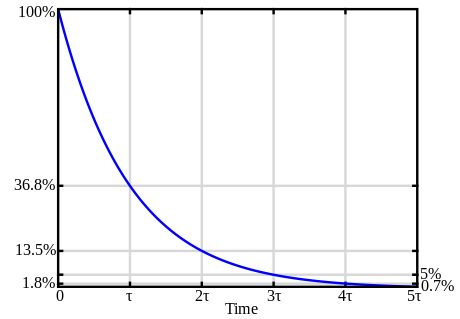
\includegraphics[scale=0.6]{RC_voltage.png}
\caption{The response of initial condition of 1st-order system}
\label{fig:RCV}
\end{figure}
\raggedright Find its time constant $\tau$ which is located at the time where the amplitude is $36.79\%$ (i.e. $e^{-1}$) of its initial value. Using the follwoing equation:
\[\tau=\frac{L}{R}\]
\[\rightarrow L=R\cdot\tau,\]
the inductance $L$ then can be derived.
\begin{itemize}
\item Required measurements: Using LabVIEW to record the response of voltage of small resistor, convert it to current data.
\end{itemize}


\subsubsection{Identifying $B$}
Apply a constant voltage, let the motor freely run, wait until its angular velocity $\omega$ reaches the steady state.\\
Since the angular velocity $\omega$ is constant, $\ddot{\theta}=\dot{\omega}=0$. Substitute that to Eq. \eqref{eqn:Mechanics}, we can get:
\[B\dot{\theta}=T\]
Then the damping of motor can be derived as follows:
\[\rightarrow B=\frac{T}{\omega}=\frac{K_t\cdot i}{omega}\]
\begin{itemize}
\item Required measurements: Using LabVIEW to read the encoder and derive its angular velocity by numerical differentiation, and using multimeter to measure the voltage $V_s$ across the small resistance to derive the current.
\end{itemize}


\subsubsection{Identifying $J$}
Apply a constant voltage, let the motor freely run, wait until its angular relovicty $\omega$ reach steady state.\\
Next, open the circuit (i.e. make $i=0$), then Eq. \eqref{eqn:Electro} becomes:
\[J\dot{\omega+B\omega=0},\]
which is also a 1st order system.
Record the response of $\omega$, which will be similar to Figure \ref{fig:RCV}, find the time constant $\tau$. Then the motor inertia $J$ can be found as follows:
\[\tau=\frac{J}{B}\]
\[\rightarrow J=\tau \cdot B\]
\begin{itemize}
\item Required measurements: Using LabVIEW to record the response of encoder, derive the response of angular velocity ($\omega$) by numerical differentiation.
\end{itemize}


%\section{Conclusion}
%``I always thought something was %fundamentally wrong with the %universe'' \citep{adams1995hitchhiker}

%\begin{figure}[h!]
%\centering
%\includegraphics[scale=1.7]{universe.jpg}
%\caption{The Universe}
%\label{fig:univerise}
%\end{figure}



\bibliographystyle{plain}
\bibliography{sample}

%\printbibliography

\end{document}
